\documentclass{article}
\usepackage{mathtools}
\usepackage{listings}
\usepackage{tikz-network}

\begin{document}
\title{CS320 Homework 7}
\author{Dustin Randall}
\maketitle

\section{Trace Dijkstra's algorithm to show the shortest path from vertex S.}
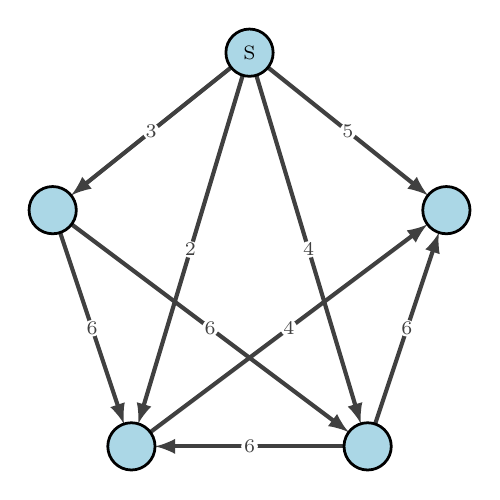
\begin{tikzpicture}
    \Vertex[x=2.5,y=5, label=S]{S}
    \Vertex[x=0,y=3]{A}
    \Vertex[x=5,y=3]{B}
    \Vertex[x=1,y=0]{C}
    \Vertex[x=4,y=0]{D}

    \Edge[Direct,label=3](S)(A)
    \Edge[Direct,label=5](S)(B)
    \Edge[Direct,label=6](A)(C)
    \Edge[Direct,label=6](A)(D)
    \Edge[Direct,label=4](C)(B)
    \Edge[Direct,label=6](D)(B)
    \Edge[Direct,label=6](D)(C)
    \Edge[Direct,label=2](S)(C)
    \Edge[Direct,label=4](S)(D)
\end{tikzpicture}


\section{Show the trace of the Bellman-Ford algorithm starting from z}
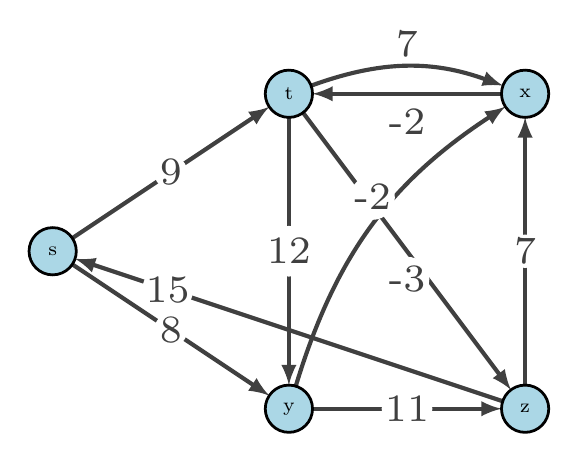
\begin{tikzpicture}
    \Vertex[x=0,y=2,label=s]{S}
    \Vertex[x=3,y=4,label=t]{T}
    \Vertex[x=6,y=4,label=x]{X}
    \Vertex[x=3,y=0,label=y]{Y}
    \Vertex[x=6,y=0,label=z]{Z}

    \Edge[fontscale=2,Direct,label=9](S)(T)
    \Edge[fontscale=2,Direct,label=8](S)(Y)
    \Edge[fontscale=2,Direct,label=15,distance=.8](Z)(S)
    \Edge[fontscale=2,Direct,label=12](T)(Y)
    \Edge[fontscale=2,Direct,label=7,position=above,bend=20](T)(X)
    \Edge[fontscale=2,Direct,label=-3,position=below](T)(Z)
    \Edge[fontscale=2,Direct,label=-2,position=below](X)(T)
    \Edge[fontscale=2,Direct,label=-2,position=above,bend=20](Y)(X)
    \Edge[fontscale=2,Direct,label=11](Y)(Z)
    \Edge[fontscale=2,Direct,label=7](Z)(X)
\end{tikzpicture}

\section{Give an $O(|V|\cdot|E|)$ algorithm for computing the transitive closure of a directed graph.}

\section{Use Floyd-Warshall algorithm to find D1, D2, D3, and D4 for the provided D0 matrix.}
\[
D^{(0)} = \begin{pmatrix}
0 & 5 & \infty & 3 \\
\infty & 0 & -1 & \infty \\
6 & \infty & 0 & \infty \\
\infty & 2 & 7 & 0
\end{pmatrix}
\]
\end{document}